% Source: graduate-coursework/Sp26/CSCE763/Course_Assignments/Exam/Midterm_Exam_solutions.tex

\documentclass[border=4pt]{standalone}
\usepackage{amsmath}
\usepackage{amssymb}
\usepackage{graphicx}
\usepackage{tikz}
\usepackage{xcolor}
\usetikzlibrary{shapes.geometric, arrows.meta, positioning, patterns, calc}

\definecolor{USC_Garnet}{HTML}{73000A}
\definecolor{USC_Sandstorm}{HTML}{FFF2E3}
\definecolor{USC_Black90}{HTML}{363636}
\definecolor{USC_Black70}{HTML}{5C5C5C}
\definecolor{USC_Black50}{HTML}{A2A2A2}
\definecolor{USC_Black10}{HTML}{ECECEC}
\definecolor{USC_Honeycomb}{HTML}{65780B}
\definecolor{USC_Atlantic}{HTML}{466A9F}
\definecolor{USC_Congaree}{HTML}{1F414D}
\definecolor{USC_Rose}{HTML}{CC2E40}

\newcommand{\problem}[1]{%
  \vspace{0.5cm}
  {\noindent\normalsize \textbf{#1}}
  \vspace{0.3cm}
}

\begin{document}
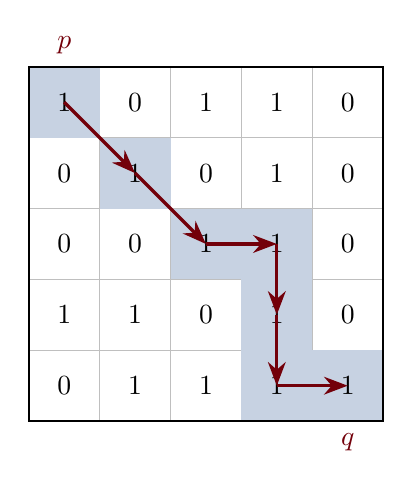
\begin{tikzpicture}[scale=0.9]
    % Draw grid
    \foreach \x in {0,1,2,3,4,5} {
        \draw[gray!50] (\x,0) -- (\x,5);
        \draw[gray!50] (0,\x) -- (5,\x);
    }

    % Highlight path pixels
    \fill[USC_Atlantic!30] (0,4) rectangle (1,5);   % (0,0)
    \fill[USC_Atlantic!30] (1,3) rectangle (2,4);   % (1,1)
    \fill[USC_Atlantic!30] (2,2) rectangle (3,3);   % (2,2)
    \fill[USC_Atlantic!30] (3,2) rectangle (4,3);   % (2,3)
    \fill[USC_Atlantic!30] (3,1) rectangle (4,2);   % (3,3)
    \fill[USC_Atlantic!30] (3,0) rectangle (4,1);   % (4,3)
    \fill[USC_Atlantic!30] (4,0) rectangle (5,1);   % (4,4)

    % Fill in values
    \node at (0.5,4.5) {1}; \node at (1.5,4.5) {0}; \node at (2.5,4.5) {1}; \node at (3.5,4.5) {1}; \node at (4.5,4.5) {0};
    \node at (0.5,3.5) {0}; \node at (1.5,3.5) {1}; \node at (2.5,3.5) {0}; \node at (3.5,3.5) {1}; \node at (4.5,3.5) {0};
    \node at (0.5,2.5) {0}; \node at (1.5,2.5) {0}; \node at (2.5,2.5) {1}; \node at (3.5,2.5) {1}; \node at (4.5,2.5) {0};
    \node at (0.5,1.5) {1}; \node at (1.5,1.5) {1}; \node at (2.5,1.5) {0}; \node at (3.5,1.5) {1}; \node at (4.5,1.5) {0};
    \node at (0.5,0.5) {0}; \node at (1.5,0.5) {1}; \node at (2.5,0.5) {1}; \node at (3.5,0.5) {1}; \node at (4.5,0.5) {1};

    % Draw arrows for m-path
    \draw[-{Stealth[length=3mm]}, USC_Garnet, very thick] (0.5,4.5) -- (1.5,3.5);  % (0,0) -> (1,1) diagonal
    \draw[-{Stealth[length=3mm]}, USC_Garnet, very thick] (1.5,3.5) -- (2.5,2.5);  % (1,1) -> (2,2) diagonal
    \draw[-{Stealth[length=3mm]}, USC_Garnet, very thick] (2.5,2.5) -- (3.5,2.5);  % (2,2) -> (2,3) horizontal
    \draw[-{Stealth[length=3mm]}, USC_Garnet, very thick] (3.5,2.5) -- (3.5,1.5);  % (2,3) -> (3,3) vertical
    \draw[-{Stealth[length=3mm]}, USC_Garnet, very thick] (3.5,1.5) -- (3.5,0.5);  % (3,3) -> (4,3) vertical
    \draw[-{Stealth[length=3mm]}, USC_Garnet, very thick] (3.5,0.5) -- (4.5,0.5);  % (4,3) -> (4,4) horizontal

    % Label p and q
    \node[USC_Garnet, font=\bfseries] at (0.5,5.3) {$p$};
    \node[USC_Garnet, font=\bfseries] at (4.5,-0.3) {$q$};

    % Draw outer border
    \draw[thick] (0,0) rectangle (5,5);
\end{tikzpicture}
\end{document}
